%		** INTRODUZIONE **

Il presente progetto si prefige como scopo quello di realizzare un sistema multi-agente per il tracciamento di target in movimento in ambiente chiuso. Gli agenti previsti sono equiparabili a telecamere, le quali hanno un numero di funzioni limitate. Lo scopo principale degli agenti � quello di tenere i target tracciati il pi� possibile, per questo viene permesso loro di "passarsi" i target quando questi si allontanano dalla loro area di visione. L'applicazione � perzonalizzabile tramite file di configurazione, i quali permettono di specificare:
\begin{itemize}
	\item l'ambiente, tramite sua rappresentazione matriciale,
	\item le stanze, definite come rettangoli,
	\item gli agenti e la loro configurazione interna.
\end{itemize}
La figura seguente mostra l'interfaccia grafica dell'applicazione.

% Figura della mappa
\begin{figure}[h]
	\centering
	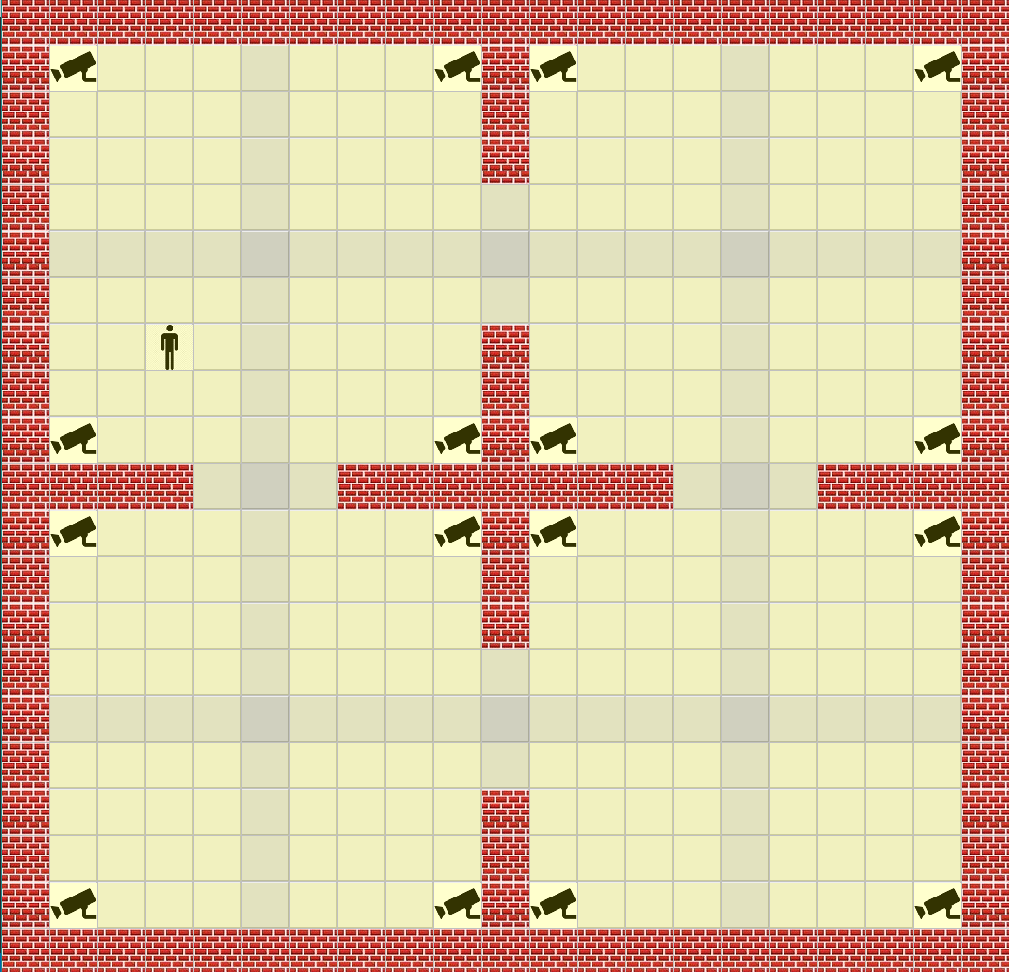
\includegraphics[width=0.5\linewidth]{mappa}
	\caption{Interfaccia grafica dell'applicazione in cui � visibile un target.}
	\label{fig:mappa}
\end{figure}